\section{Aufbau}
\begin{figure}
	\centering
	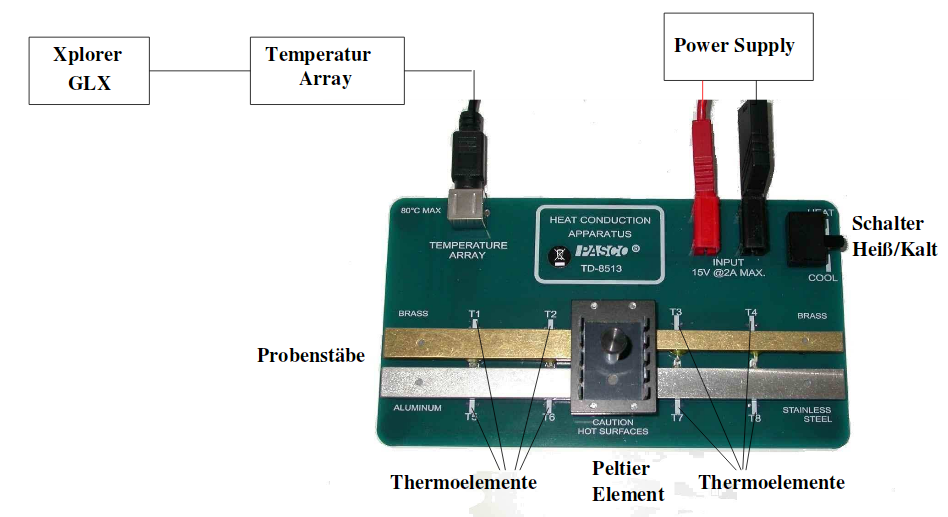
\includegraphics[width=\linewidth-100pt,height=\textheight-100pt,keepaspectratio]{content/Bilder/aufbau204.png}
	\caption{ Messaufbau zur Aufnahme von Wärmeleitungkurven\cite{V204}.}
	\label{fig:Aufbau}
\end{figure}
Der Messaufbau besteht aus einer rechteckigen Platte, in dessen Mitte
 ein Peretiergerät angebracht ist. Das Peretiergerät wird über einen Energiequelle
  mit Energie versorgt. Zu beiden Seiten des Gerätes sind 4 Stäbe aus unterschiedlichen
  Metallen angebracht, welche über das Peretiergerät mittels eines Schalters entweder erwärmt oder abgekühlt
   werden können.
   Es sind ein breiter und ein schmaler Messingstab, ein
   Aluminiumstab sowie ein Stab aus Edelstahl verbaut. An jedem Stab sind zwei
   Thermoelemente im Abstand von $\SI{3}{\centi\meter}$ angebracht. Die gemessenen
   Temperaturen aller 8 Stellen werden über einen GLX Datenlogger an einen Xplorer GLX
   weitergegeben. Sie sind über die Nummerierung auf der Platte nach Abb.
    \ref{fig:Aufbau} identifizierbar. Auf dem Xplorer GLX können die aufgenommenen Temperaturkurven erstellt,
   bearbeitet und über einen Drucker ausgedruckt werden.
